Neste último capítulo trataremos de forma pincelada de um método de ataque
ao problema de se provar a continuidade de $\tep$ em $\pce$ em mais dimensões
do que duas. Neste caso, não temos nem a auto-dualidade da rede
hipercúbica nem conhecemos (ou esperamos algum dia conhecer) o valor exato
de $\pce$. Ambos conhecimentos foram úteis em $d=2$ (Capítulo~\ref{chp:bid}).

A idéia será relacionar a ocorrência de percolação a um evento {\em em volume
finito}, cuja probabilidade, sendo contínua (pois as probabilidades de todos
tais eventos são polinômios em $p$), nos permitirá concluir que, se há 
percolação para $p$, então há também para $p-\eps$ com $\eps>0$ 
suficientemente pequeno.

O método é chamado de {\em renormalização}. A versão a ser esboçada, que chamaremos
renormalização {\em estática}, não foi ainda realizada com rigor em modelos
de percolação (uma prova para a Proposi\c cão~\ref{pro:ren2} abaixo
ainda não
foi feita), mas técnicas de renormalização {\em dinâmica} muito similares
foram aplicadas
com sucesso para percolação em semi-espaços de $\bbz^d$, $d\geq3$ 
\cite{kn:BGN}. O problema da continuidade no ponto crítico
em $\zd$ inteiro permanece aberto para valores intermediários de $d$ entre
$2$ e $d_0$, este último o menor valor para o qual Hara e Slade \cite{kn:HS} podem
aplicar sua {\em expansão em laços} e obter a continuidade a partir daí, entre outros 
resultados ($d_0$ estava em 19 segundo as últimas notícias,
mas não se espera que possa vir abaixo de 7).

Para $0\leq K\leq L$, considere a partição de $\zd$ em cubos concêntricos 
de lado $2K$ e $2L$ como na figura abaixo e seja $\akl$ o evento em que
existe um caminho aberto dentro dos dois cubos grandes conectando a superfície
dos dois cubos menores (vide Figura~\ref{fig:fren1}).

\bef
%\input fren1
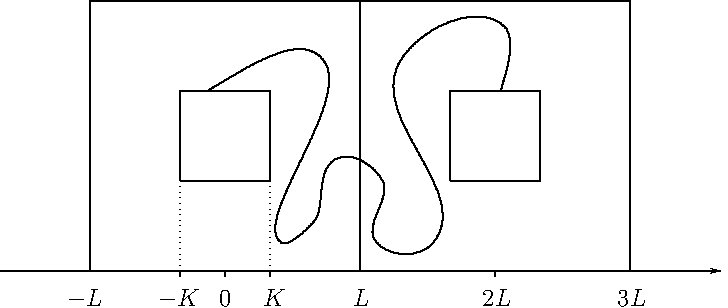
\includegraphics{fren1}
\caption{O evento $\akl$}
\label{fig:fren1}
\eef

Para garantir interconexão, precisamos intersectar $\akl$ com outro e\-ven\-to
$$\bkl=\bklu\cap\bkld,$$
em que $\bkli$, $i=1,2$, é o evento de que todos os sítios do cubo menor $i$, que
estiverem ligados por caminhos abertos à fronteira do cubo grande respectivo,
estarão conectados entre si por caminhos abertos dentro do cubo grande.

Seja $\aklt=\akl\cap\bkl$.

\vs

\bpro
\label{pro:ren1}
Seja $\rkl=\p(\aklt).$ Existe $\ls\in(0,1)$ tal que se (para algum $0\leq
K\leq L$ e $0<p<1$) $\rklp>\ls$, então $\tep>0$.
\epro
Um argumento para a validade deste resultado será esboçado adiante.

\vs

\bpro[Conjectura]
\label{pro:ren2}
Se, para algum $p'\in(0,1)$, $\tepl>0$, então
\beq
\label{eq:ren1}
\sup_K\liminf_{L\to\infty}P_{p'}(\akl)=1.
\eeq
\epro

\vs

\bte
\label{teo:ren}
Se a Proposição~\ref{pro:ren2} conjecturada for verdadeira, então $$\tepc=0.$$
\ete

\noindent{\bf Prova do teorema.}

Primeiro mostraremos que a Proposição~\ref{pro:ren2} conjecturada implica que
se $\tepl>0$, então 
\beq
\label{eq:ren2}
\sup_K\liminf_{L\to\infty}\rklpl=1
\eeq
(portanto $\rklpl>\ls$ para algum $K$ e $L$).

De fato, para cada $K$ fixo, $$\lim_{L\to\infty}\ppl(\bkli)=1$$
para $i=1,2$, pois de outra forma haveria probabilidade positiva de que 2
sítios do cubo menor estivessem em aglomerados infinitos disjuntos.
Logo $$\lim_{L\to\infty}\ppl(\bkl)=1$$ do que se conclui que
$$\lim_{L\to\infty}\ppl(\aklt)=\lim_{L\to\infty}\ppl(\akl)=1.$$

Agora suponha que, para algum $p'$, $\tepl>0$. Pelo argumento acima podemos
escolher $K_0$ e $L_0$ tais que $\rko>\ls$. Mas $\rkop$ é um polinômio em
$p$. Logo $$\rkoe>\ls$$ para algum $\eps$ positivo. Pela Proposição~\ref{pro:ren1}
$$\teple>0.$$

Temos portanto que $\tepl>0$ implica que $\teple>0$ para algum $\eps>0$.
Logo $\tepc$ não pode ser positivo, pois isto implicaria em $\tep$ positivo
para algum $p<\pce$, o que contradiz a definição de $\pce$. $\bo$

\vs

\noindent{\bf (Esboço de) Prova da Proposição~\ref{pro:ren1} (em $d=3$).}

Considere uma rede {\em renormalizada} isomórfica a $\zt$ na qual cada sítio
corresponde a um cubo $2L\times2L\times2L$ em $\bbz^3$, como na
Figura~\ref{fig:fren2}. Declare um elo
{\em renormalizado} aberto se $\aklt(e)$ ocorrer. 

\bef
%\input fren2
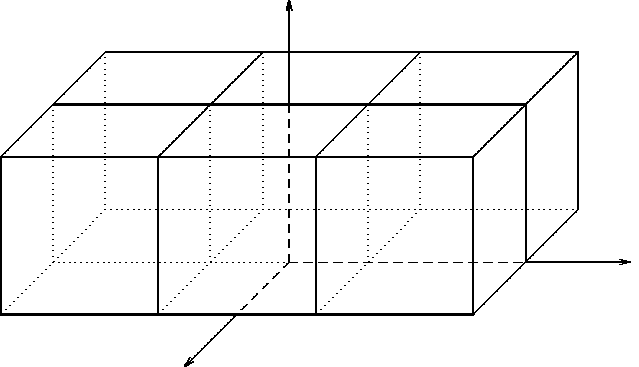
\includegraphics{fren2}
\caption{Parte da rede $\zt$ renormalizada.}
\label{fig:fren2}
\eef

Teremos então um modelo de percolação {\em dependente} na rede renormalizada
com uma medida de probabilidade $\ppt$ tal que 
$$\ppt(\mbox{$e$ está aberto})=\rkl.$$

Precisamos mostrar que existe $\ls\in(0,1)$ tal que se $\rkl$ for maior do 
que $\ls$, então
percolação dependente ocorre na rede renormalizada. Se isto ocorrer,
obviamente percolação independente ocorrerá na rede original.

A prova de que percolação dependente ocorre em $\zt$ renormalizada pode ser feita 
pelo mesmo argumento de Peierls na prova da Proposição~\ref{prop:trans2}
(a partir dos circuitos nos elos duais de $\zt$)
com a única pequena modificação de que a medida nos elos não é mais
independente, mas apenas {\em localmente} dependente. Deixamos os detalhes 
para o leitor. $\bo$
